% !TeX spellcheck = en_US
\addsection{Components}{\skills/luck.png}

This guide provides a visual overview of all components included in every expansion. For detailed information, including exact quantities and images of each individual component, please refer to the Archon's official content guide.

\begin{figure}[H]
  \centering
  \hfill
  \begin{subfigure}[c]{0.25\linewidth}
    \centering
    \includegraphics[width=\linewidth]{\images/map-tile-back.png}
    \caption{\textbf{\pagelink{Map}{Map Tile}}}
  \end{subfigure}
  \hfill
  \begin{subfigure}[c]{0.25\linewidth}
    \begin{expansionmini}{cove}
      \centering
      \vspace{0.5em}
      \includegraphics[width=0.7\linewidth]{\images/map-tile-sea.png}
      \caption{\textbf{\pagelink{Sea Map Tiles}{Sea Map Tile}}}
    \end{expansionmini}
  \end{subfigure}
  \hfill
  \begin{subfigure}[c]{0.25\linewidth}
    \begin{expansionmini}{stronghold}
      \centering
      \vspace{0.5em}
      \includegraphics[width=0.7\linewidth]{\images/map-tile-sub.png}
      \caption{\textbf{\pagelink{Subterranean Map Tiles}{Subterranean Map Tile}}}
    \end{expansionmini}
  \end{subfigure}
  \hfill
  ~
\end{figure}

\begin{figure}[H]
  \centering
  \hfill
  \begin{subfigure}[c]{0.15\linewidth}
    \centering
    \includegraphics[width=0.6\linewidth]{\images/movement-tokens.png}
    \caption{\textbf{\pagelink{Movement}{Movement Tokens}}}
  \end{subfigure}
  \hfill
  \begin{subfigure}[c]{0.17\linewidth}
    \begin{expansionmini}{navalbattles}
      \vspace{3mm}
      \centering
      \includegraphics[width=0.8\linewidth]{\map_locations/creature-bank.png}
      \caption{\textbf{\pagelink{Creature Bank Tokens}{Creature Bank Token}}}
    \end{expansionmini}
  \end{subfigure}
  \hfill
  \begin{subfigure}[c]{0.15\linewidth}
    \begin{expansionmini}{cove}
      \vspace{3mm}
      \centering
      \includegraphics[width=0.6\linewidth]{\map_locations/whirlpool.png}
      \caption{\textbf{\pagelink{Whirlpool Tokens}{Whirlpool Token}}}
    \end{expansionmini}
  \end{subfigure}
  \hfill
  \begin{subfigure}[c]{0.15\linewidth}
    \begin{expansionmini}{conflux}
      \vspace{3mm}
      \centering
      \includegraphics[width=0.6\linewidth]{\map_locations/monolith_token.png}
      \caption{\textbf{\pagelink{Monolith Tokens}{Monolith Token}}}
    \end{expansionmini}
  \end{subfigure}
  \hfill
  \begin{subfigure}[c]{0.16\linewidth}
    \begin{expansionmini}{stronghold}
      \centering
      \vspace*{0.5em}
      \includegraphics[width=0.75\linewidth]{\map_locations/subterranean_gate_token.png}
      \caption{\textbf{\pagelink{Subterranean Gate}{Subterranean Gate}}}
    \end{expansionmini}
  \end{subfigure}
  \hfill
  ~
\end{figure}

\begin{figure}[H]
  \centering
  \begin{subfigure}[c]{0.3\linewidth}
    \includegraphics[width=\linewidth]{\images/town-empty.png}
    \caption{\textbf{\pagelink{Town}{Town Board}}}
  \end{subfigure}
  ~
  \begin{subfigure}[c]{0.3\linewidth}
    \centering
    \includegraphics[width=0.25\linewidth]{\images/town-tile-1.png}
    \includegraphics[width=0.25\linewidth]{\images/town-tile-2.png}
    \includegraphics[width=0.25\linewidth]{\images/town-tile-3.png}
    \caption{\textbf{\pagelink{Town}{Building Tiles}}}
  \end{subfigure}
  ~
  \begin{subfigure}[c]{0.22\linewidth}
    \begin{expansionmini}{stretchgoals2}
      \centering
      \begin{tikzpicture}
        \node at (0, 0) {\includegraphics[width=0.6\linewidth]{\cards/town-card-back.png}};
        \node at (1.5, 0.1) {\includegraphics[width=0.6\linewidth]{\cards/town-card.png}};
      \end{tikzpicture}
      \caption{\textbf{\pagelink{Town Card}{Town card}}}
    \end{expansionmini}
  \end{subfigure}
  ~
\end{figure}

\begin{figure}[H]
  \centering
  \begin{subfigure}[c]{0.18\linewidth}
    \centering
    \includegraphics[width=\linewidth]{\images/gold-tokens.png}
    \caption{\textbf{\pagelink{Resources}{Gold Tokens}}}
  \end{subfigure}
  \begin{subfigure}[c]{0.12\linewidth}
    \centering
    \includegraphics[width=0.6\linewidth]{\images/building-materials-token.png}
    \caption{\textbf{\pagelink{Resources}{Building Materials}}}
  \end{subfigure}
  \begin{subfigure}[c]{0.12\linewidth}
    \centering
    \includegraphics[width=0.6\linewidth]{\images/valuables-token.png}
    \caption{\textbf{\pagelink{Resources}{Valuables Token}}}
  \end{subfigure}
  \begin{subfigure}[c]{0.12\linewidth}
    \centering
    \includegraphics[width=5em]{\images/build.png}
    \caption{\textbf{\pagelink{Town Actions}{Build Token}} \iftoggle{printable}{}{\phantom{Population}}}
  \end{subfigure}
  \begin{subfigure}[c]{0.13\linewidth}
    \centering
    \includegraphics[width=5em]{\images/population.png}
    \caption{\textbf{\pagelink{Town Actions}{Population Token}} \iftoggle{printable}{}{\phantom{Population}}}
  \end{subfigure}
  \begin{subfigure}[c]{0.12\linewidth}
    \centering
    \includegraphics[width=5em]{\images/spells.png}
    \caption{\textbf{\pagelink{Town Actions}{\mbox{Spell Book} Token}} \iftoggle{printable}{}{\phantom{Population}}}
  \end{subfigure}
\end{figure}

\clearpage

\begin{figure}[H]
  \centering
  \begin{subfigure}[c]{0.3\linewidth}
    \includegraphics[width=\linewidth]{\images/hero.png}
    \caption{\textbf{\pagelink{Herocard}{Hero Board}}}
  \end{subfigure}
  ~
  \begin{subfigure}[c]{0.4\linewidth}
    \centering
    \includegraphics[width=\linewidth]{\images/hero-minis.png}
    \caption{\textbf{Hero Miniatures}}
  \end{subfigure}
\end{figure}

\begin{figure}[H]
  \centering
  \begin{subfigure}[c]{0.22\linewidth}
    \centering
    \begin{tikzpicture}
      \node at (0, 0) {\includegraphics[width=0.7\linewidth]{\cards/astrolog-back.png}};
      \node at (0.7, 1.2) {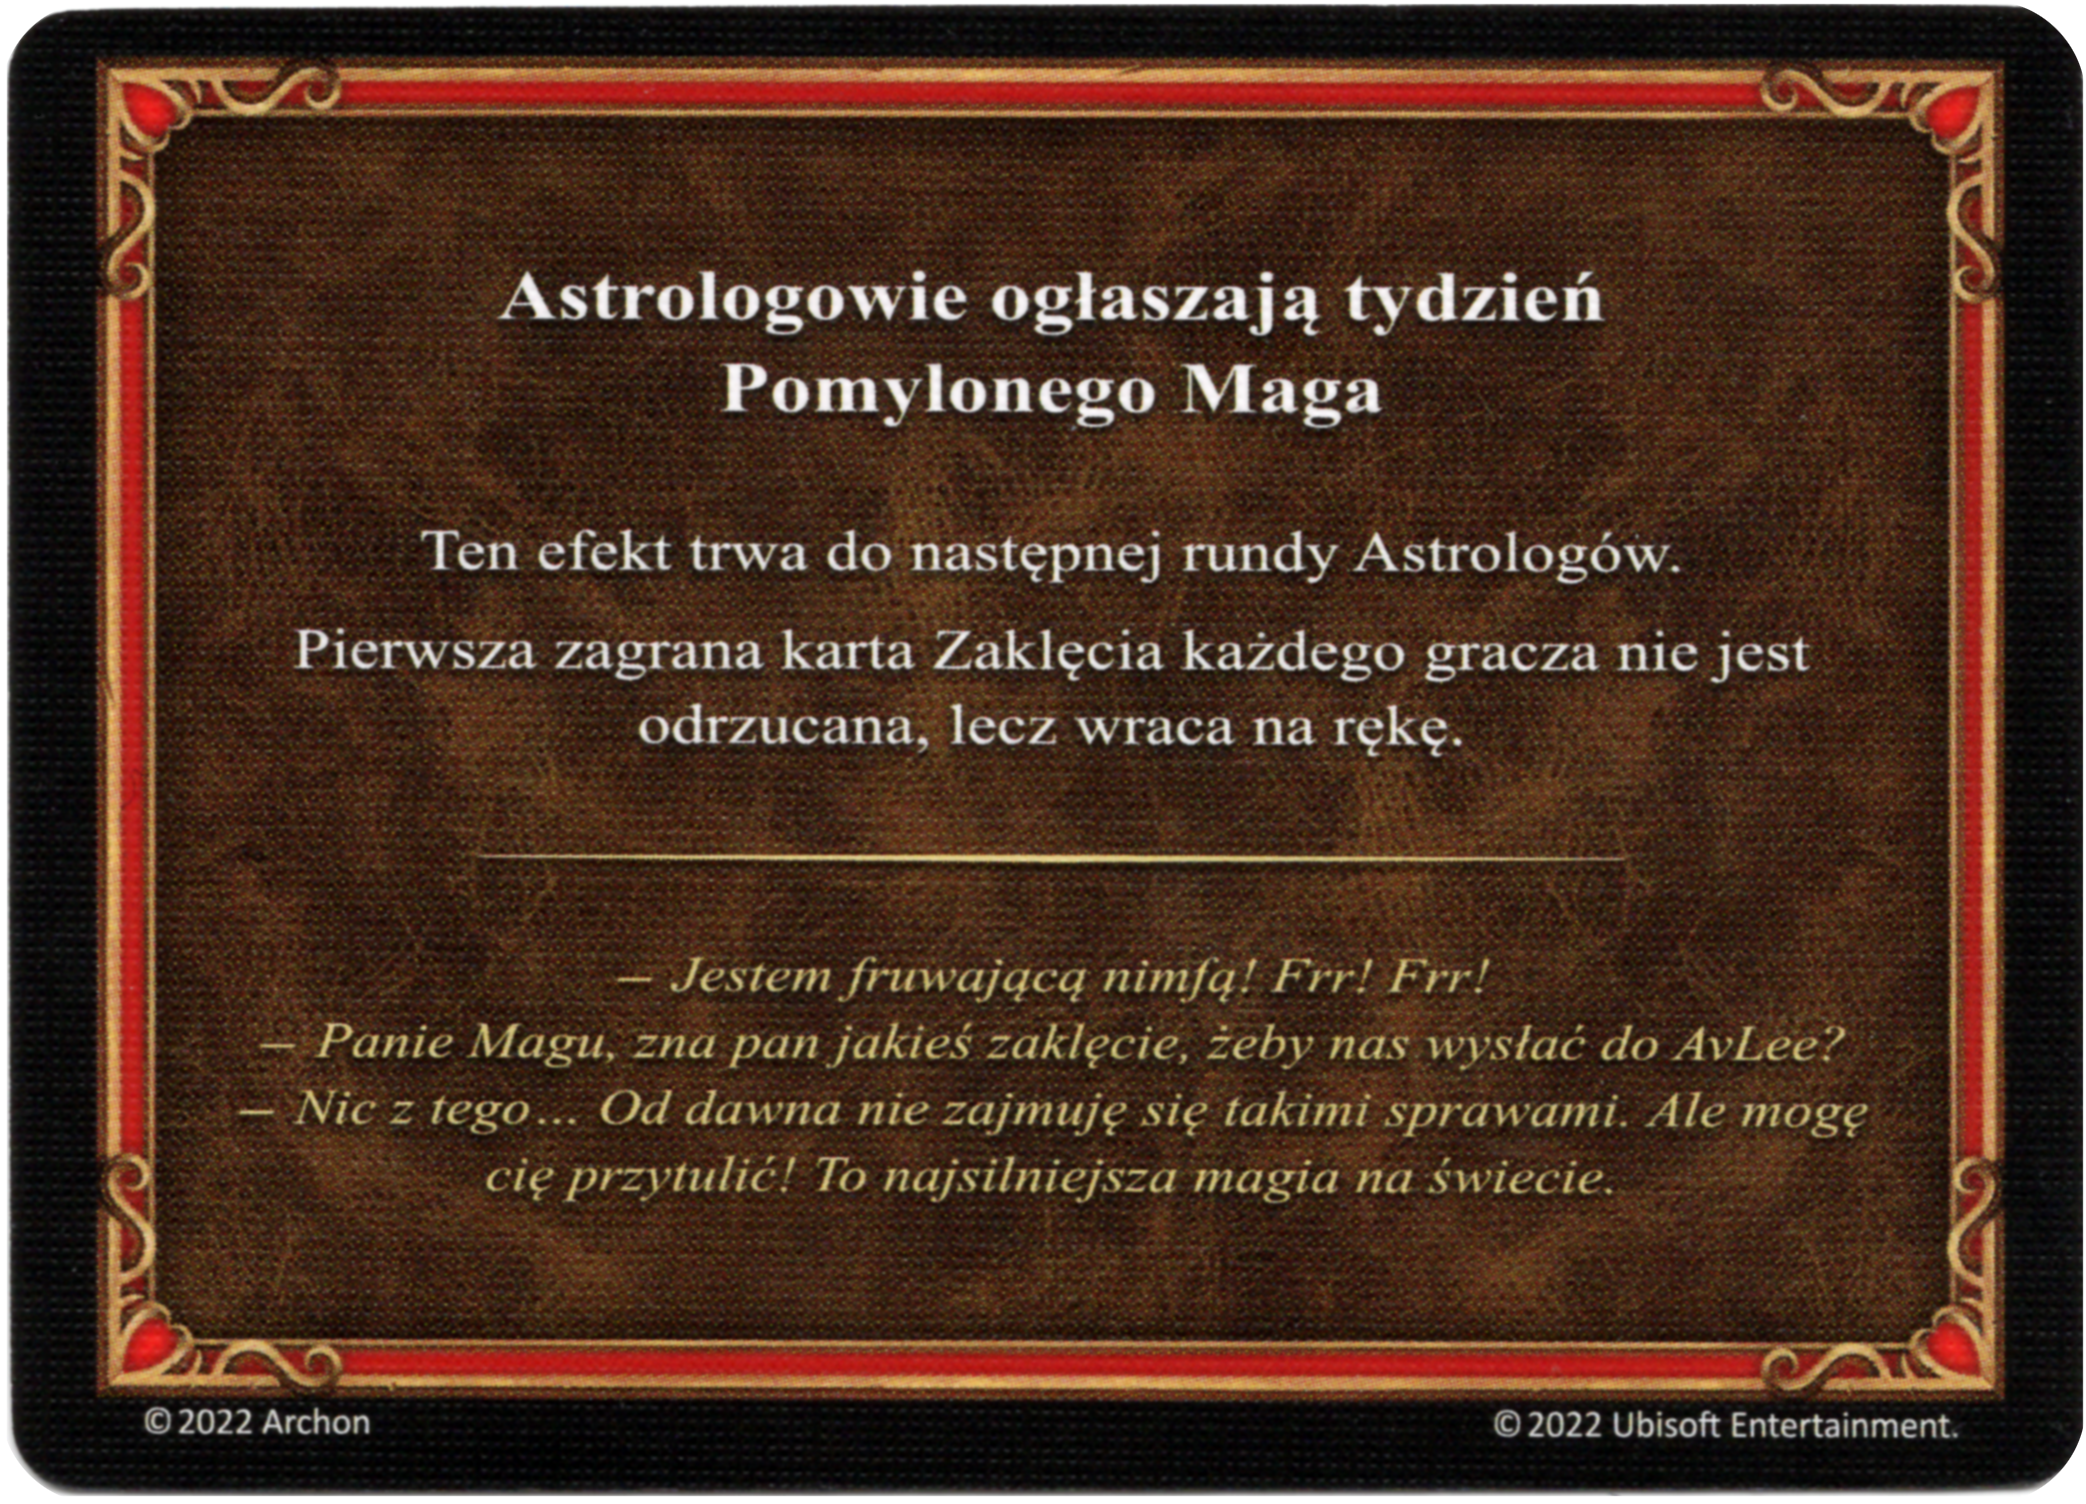
\includegraphics[width=0.7\linewidth]{\cards/astrolog.png}};
    \end{tikzpicture}
    \caption{\textbf{\pagelink{Rounds}{Astrologers Proclaim card}}}
  \end{subfigure}
  ~
  \begin{subfigure}[c]{0.22\linewidth}
    \begin{expansionmini}{fortress}
      \centering
      \begin{tikzpicture}
        \node at (0, 0) {\includegraphics[width=0.8\linewidth]{\cards/event-back.png}};
        \node at (0.7, 1.2) {\includegraphics[width=0.8\linewidth]{\cards/event.png}};
      \end{tikzpicture}
      \caption{\textbf{\pagelink{Events}{Event card}}}
    \end{expansionmini}
  \end{subfigure}
  ~
  \begin{subfigure}[c]{0.22\linewidth}
    \begin{expansionmini}{battlefield}
      \centering
      \vspace{0.5em}
      \includegraphics[width=\linewidth]{\cards/adventure.png}
      \caption{\textbf{\pagelink{Adventure Cards}{Adventure card}}}
    \end{expansionmini}
  \end{subfigure}
  ~
  \begin{subfigure}[c]{0.23\linewidth}
    \begin{expansionmini}{stretchgoals2}
      \centering
      \begin{tikzpicture}
        \node at (0, 0) {\includegraphics[width=0.6\linewidth]{\cards/pandora-back.png}};
        \node at (1.5, 0.1) {\includegraphics[width=0.6\linewidth]{\cards/pandora.png}};
      \end{tikzpicture}
    \caption{\textbf{\pagelink{Pandora Card}{Pandora's Box card}}}
    \end{expansionmini}
  \end{subfigure}
\end{figure}

\begin{figure}[H]
  \centering
  \hfill
  \begin{subfigure}[c]{0.15\linewidth}
    \centering
    \includegraphics[width=0.8\linewidth]{\images/faction-cubes.png}
    \caption{\textbf{Faction Cubes}}
  \end{subfigure}
  \hfill
  \begin{subfigure}[c]{0.15\linewidth}
    \centering
    \includegraphics[width=\linewidth]{\images/black-cubes.png}
    \caption{\textbf{Black Cubes}}
  \end{subfigure}
  \hfill
  \begin{subfigure}[c]{0.12\linewidth}
    \centering
    \includegraphics[width=0.8\linewidth]{\images/grail.png}
    \caption{\textbf{\pagelink{Grail}{Grail Token}}}
  \end{subfigure}
  \hfill
  \begin{subfigure}[c]{0.15\linewidth}
    \begin{expansionmini}{navalbattles}
      \centering
      \vspace{0.5em}
      \includegraphics[width=0.6\linewidth]{\images/crown-token.png}
      \caption{\textbf{\pagelink{Empowered Ability Token}{Empowered Ability Token}}}
    \end{expansionmini}
  \end{subfigure}
  \hfill
  ~
\end{figure}

\begin{figure}[H]
  \centering
  \begin{subfigure}[c]{0.4\linewidth}
    \centering
    \includegraphics[width=0.8\linewidth]{\images/round-tracker.png}
    \caption{\textbf{\pagelink{Rounds}{Round Tracker}}}
  \end{subfigure}
  \begin{subfigure}[c]{0.15\linewidth}
    \centering
    \includegraphics[width=0.7\linewidth]{\images/attack_die.png}
    \caption{\textbf{\pagelink{Combatterminology}{Attack Dice}} \\\phantom{Population}}
  \end{subfigure}
  \begin{subfigure}[c]{0.15\linewidth}
    \centering
    \includegraphics[width=\linewidth]{\images/treasure_die.png}
    \caption{\textbf{\pagelink{Treasure Die}{Treasure Dice}}}
  \end{subfigure}
  \begin{subfigure}[c]{0.15\linewidth}
    \centering
    
\includegraphics[width=0.8\linewidth]{\images/resource_die.png}
    \caption{\textbf{\pagelink{Resources}{Resource Dice}}}
  \end{subfigure}
\end{figure}

\vspace*{-1em}
\begin{figure}[H]
  \centering
  \begin{subfigure}[c]{0.9\linewidth}
    \centering
    \begin{tikzpicture}

      % background
      \node[opacity=0.75] at (6.7, 0.7) {\includegraphics[scale=1.2]{\images/unitmini-evileye.png}};
      \node[opacity=0.75] at (-3.9, 1.0) {\includegraphics[scale=1.4]{\images/unitmini-dwarf.png}};
      \node[opacity=0.75] at (-0.9, 0.66) {\includegraphics[scale=1.4]{\images/unitmini-naga.png}};
      \node[opacity=0.75] at (3.1, 0.7) {\includegraphics[scale=1.4]{\images/unitmini-lich.png}};
      \node[opacity=0.75] at (1, 1.1) {\includegraphics[scale=1.4]{\images/unitmini-archangel.png}};
      \node[opacity=0.75, xscale=-1] at (-2.6, 1) {\includegraphics[scale=1.2]{\images/unitmini-troglodyte.png}};
      % foreground
      \node at (-3.5, 0) {\includegraphics[scale=0.9]{\images/unitmini-magicelemental.png}};
      \node at (-1.6, -0.4) {\includegraphics[scale=0.9]{\images/unitmini-seaman.png}};
      \node at (2, -0.1) {\includegraphics[scale=0.9]{\images/unitmini-archdevil.png}};
      \node at (0, 0.15) {\includegraphics[scale=1.1]{\images/unitmini-cyclops.png}};
      \node at (5.1, 0.6) {\includegraphics[scale=0.7]{\images/unitmini-haspid.png}};
    \end{tikzpicture}
    \caption{\textbf{\pagelink{Miniatures}{Unit Miniatures}}\\\textit{(Not included in the core game)}}
  \end{subfigure}
\end{figure}

\clearpage

\begin{figure}[H]
  \centering
  \begin{subfigure}[c]{0.23\linewidth}
    \centering
    \begin{tikzpicture}
      \node at (0, 0) {\includegraphics[width=0.6\linewidth]{\cards/mmback.png}};
      \node at (1.5, 0.1) {\includegraphics[width=0.6\linewidth]{\cards/spell.png}};
    \end{tikzpicture}
    \caption{\textbf{\pagelink{spells}{Spell card}}}
  \end{subfigure}
  \begin{subfigure}[c]{0.23\linewidth}
    \centering
    \begin{tikzpicture}
      \node at (0, 0) {\includegraphics[width=0.6\linewidth]{\cards/mmback.png}};
      \node at (1.5, 0.1) {\includegraphics[width=0.6\linewidth]{\cards/artifact-front.png}};
    \end{tikzpicture}
    \caption{\textbf{\pagelink{Artifact}{Artifact card}}}
  \end{subfigure}
  \begin{subfigure}[c]{0.23\linewidth}
    \centering
    \begin{tikzpicture}
      \node at (0, 0) {\includegraphics[width=0.6\linewidth]{\cards/mmback.png}};
      \node at (1.5, 0.1) {\includegraphics[width=0.6\linewidth]{\cards/ability-offense.png}};
    \end{tikzpicture}
    \caption{\textbf{\pagelink{Ability}{Ability card}}}
  \end{subfigure}
  \begin{subfigure}[c]{0.23\linewidth}
    \centering
    \begin{tikzpicture}
      \node at (0, 0) {\includegraphics[width=0.6\linewidth]{\cards/mmback.png}};
      \node at (1.5, 0.1) {\includegraphics[width=0.6\linewidth]{\cards/statistic.png}};
    \end{tikzpicture}
    \caption{\textbf{\pagelink{Statistic}{Statistic card}}}
  \end{subfigure}
\end{figure}

\begin{figure}[H]
  \centering
  \begin{subfigure}[c]{0.23\linewidth}
    \centering
    \begin{tikzpicture}
      \node at (0, 0) {\includegraphics[width=0.6\linewidth]{\cards/mmback.png}};
      \node at (1.5, 0.1) {\includegraphics[width=0.6\linewidth]{\cards/specialty.png}};
    \end{tikzpicture}
    \caption{\textbf{\pagelink{Specialty}{Hero Specialty card}}}
  \end{subfigure}
  ~
  \begin{subfigure}[c]{0.22\linewidth}
    \begin{expansionmini}{stronghold}
      \centering
      \begin{tikzpicture}
        \node at (0, 0) {\includegraphics[width=0.6\linewidth]{\cards/mmback.png}};
        \node at (1.5, 0.1) {\includegraphics[width=0.6\linewidth]{\cards/test_spellscroll.png}};
      \end{tikzpicture}
      \caption{\textbf{\pagelink{Spell Scroll Cards}{Spell Scroll card}}}
    \end{expansionmini}
  \end{subfigure}
  ~
  \begin{subfigure}[c]{0.23\linewidth}
    \begin{expansionmini}{navalbattles}
      \centering
      \begin{tikzpicture}
        \node at (0, 0) {\includegraphics[width=0.6\linewidth]{\cards/mmback.png}};
        \node at (1.5, 0.1) {\includegraphics[width=0.6\linewidth]{\cards/ability-offense-empowered.png}};
      \end{tikzpicture}
      \caption{\textbf{\pagelink{Empowered Ability}{Empowered Ability card}}}
    \end{expansionmini}
  \end{subfigure}
  ~
  \begin{subfigure}[c]{0.23\linewidth}
    \begin{expansionmini}{inferno}
      \centering
      \begin{tikzpicture}
        \node at (0, 0) {\includegraphics[width=0.6\linewidth]{\cards/mmback.png}};
        \node at (1.5, 0.1) {\includegraphics[width=0.6\linewidth]{\cards/empowered_statistic.png}};
      \end{tikzpicture}
      \caption{\textbf{\pagelink{Empowered Statistic}{Empowered Statistic card}}}
    \end{expansionmini}
  \end{subfigure}
\end{figure}

\begin{figure}[H]
  \centering
  \begin{subfigure}[c]{0.23\linewidth}
    \centering
    \begin{tikzpicture}
      \node at (0, 0) {\includegraphics[width=0.6\linewidth]{\cards/unit-pack.png}};
      \node at (1.5, 0.1) {\includegraphics[width=0.6\linewidth]{\cards/unit-few.png}};
    \end{tikzpicture}
    \caption{\textbf{\pagelink{Units}{Faction Unit card}}}
  \end{subfigure}
  ~
  \begin{subfigure}[c]{0.23\linewidth}
    \begin{expansionmini}{conflux}
      \centering
      \begin{tikzpicture}
        \node at (0, 0) {\includegraphics[width=0.6\linewidth]{\cards/unit-summoned-pack.png}};
        \node at (1.5, 0.1) {\includegraphics[width=0.6\linewidth]{\cards/unit-summoned-few.png}};
      \end{tikzpicture}
      \caption{\textbf{\pagelink{Summoning}{Summoned Unit card}}}
    \end{expansionmini}
  \end{subfigure}
  ~
  \begin{subfigure}[c]{0.23\linewidth}
    \begin{expansionmini}{navalbattles}
      \centering
      \begin{tikzpicture}
        \node at (0, 0) {\includegraphics[width=0.6\linewidth]{\cards/creature-bank-back.png}};
        \node at (1.5, 0.1) {\includegraphics[width=0.6\linewidth]{\cards/creature-bank.png}};
      \end{tikzpicture}
      \caption{\textbf{\pagelink{Creature Banks Rules}{Creature Bank Unit card}}}
    \end{expansionmini}
  \end{subfigure}
  ~
  \begin{subfigure}[c]{0.23\linewidth}
    \begin{expansionmini}{rampart,cove}
      \centering
      \begin{tikzpicture}
        \node at (0, 0) {\includegraphics[width=0.6\linewidth]{\cards/mmback.png}};
        \node at (1.5, 0.1) {\includegraphics[width=0.6\linewidth]{\cards/war_machine.png}};
      \end{tikzpicture}
      \caption{\textbf{\pagelink{War Machines}{War Machine card}}}
    \end{expansionmini}
  \end{subfigure}
\end{figure}

\begin{figure}[H]
  \centering
  \hfill
  \begin{subfigure}[c]{0.23\linewidth}
    \centering
    \begin{tikzpicture}
      \node at (0, 0) {\includegraphics[width=0.6\linewidth]{\cards/neutral-back.png}};
      \node at (1.5, 0.1) {\includegraphics[width=0.6\linewidth]{\cards/neutral-front.png}};
    \end{tikzpicture}
    \caption{\textbf{\pagelink{Neutral Units}{Neutral Unit card}}}
  \end{subfigure}
  \hfill
  \begin{subfigure}[c]{0.23\linewidth}
    \centering
    \begin{tikzpicture}
      \node at (0, 0) {\includegraphics[width=0.6\linewidth]{\cards/arrow_tower_back.png}};
      \node at (1.5, 0.1) {\includegraphics[width=0.6\linewidth]{\cards/arrow_tower.png}};
    \end{tikzpicture}
    \caption{\textbf{\pagelink{Walls}{Arrow Tower card}}}
  \end{subfigure}
  \hfill
  \begin{subfigure}[c]{0.23\linewidth}
    \centering
    \includegraphics[width=\linewidth]{\cards/gate.png}
    \caption{\textbf{\pagelink{Walls}{Gate, Walls cards}}}
  \end{subfigure}
  \hfill
  \begin{subfigure}[c]{0.23\linewidth}
    \centering
    \includegraphics[width=\linewidth]{\cards/aiback.png}
    \caption{\textbf{\pagelink{AIrules}{AI card}}}
  \end{subfigure}
  \hfill
  ~
\end{figure}

\clearpage

\vspace*{-1em}
\begin{figure}[H]
  \centering
  \begin{subfigure}[b]{0.4\linewidth}
    \includegraphics[width=\linewidth]{\images/combat_board.png}
    \caption{\textbf{\pagelink{Combat}{Combat Board}}}
  \end{subfigure}
  \hspace*{5em}
  ~
  \begin{subfigure}[b]{0.3\linewidth}
    \begin{expansion}{battlefield}
      \includegraphics[width=\linewidth]{\images/battlefield-alone.png}
      \caption{\textbf{\pagelink{Battlefield Combat}{Battlefield Board}}}
    \end{expansion}
  \end{subfigure}
\end{figure}

\vspace*{-1em}
\begin{figure}[H]
  \centering
  \begin{subfigure}[c]{0.17\linewidth}
    \centering
    \includegraphics[width=4.5em]{\images/paralysis-defense.png}
    \caption{\textbf{\hyperlink{Paralysis}{Paralysis}/ \pagelink{Defend}{Defense} Token}}
  \end{subfigure}
  \begin{subfigure}[c]{0.1\linewidth}
    \centering
    \includegraphics[width=3em]{\images/damage-token.png}
    \caption{\textbf{\pagelink{combatround}{Damage Token}}}
  \end{subfigure}
  ~
  \begin{subfigure}[c]{0.15\linewidth}
    \begin{expansionmini}{navalbattles}
      \centering
      \vspace{0.5em}
      \includegraphics[width=0.5\linewidth]{\images/stack-token.png}
      \caption{\textbf{\pagelink{Stack Tokens}{Stack Token}}}
    \end{expansionmini}
  \end{subfigure}
  ~
  \begin{subfigure}[c]{0.15\linewidth}
    \begin{expansionmini}{cove}
      \centering
      \vspace{0.5em}
      \includegraphics[width=0.5\linewidth]{\images/weakness-token.png}
      \caption{\textbf{\pagelink{Weakness Token}{Weakness Token}}}
    \end{expansionmini}
  \end{subfigure}
  ~
  \begin{subfigure}[c]{0.15\linewidth}
    \begin{expansionmini}{stronghold}
      \centering
      \vspace{0.5em}
      \includegraphics[width=0.5\linewidth]{\images/attack-token.png}
      \caption{\textbf{\pagelink{Attack Token}{Attack Token}}}
    \end{expansionmini}
  \end{subfigure}
\end{figure}

\vspace*{-1.5em}
\begin{figure}[H]
  \centering
  \begin{subfigure}[c]{0.15\linewidth}
    \begin{expansionmini}{stronghold}
      \centering
      \vspace{0.5em}
      \begin{tikzpicture}
        \node at (0, 0) {\includegraphics[width=0.5\linewidth]{\images/quicksand-token-2.png}};
        \node at (0.7, 0) {\includegraphics[width=0.5\linewidth]{\images/quicksand-token.png}};
      \end{tikzpicture}
      \caption{\textbf{\pagelink{Quicksand Token}{Quicksand Token}}}
    \end{expansionmini}
  \end{subfigure}
  ~
  \begin{subfigure}[c]{0.18\linewidth}
    \begin{expansionmini}{cove}
      \centering
      \vspace{0.5em}
      \begin{tikzpicture}
        \node at (0, 0.2) {\includegraphics[width=0.7\linewidth]{\images/clone-token-2.png}};
        \node at (0.7, 0) {\includegraphics[width=0.5\linewidth]{\images/clone-token.png}};
      \end{tikzpicture}
      \caption{\textbf{\pagelink{Clone Token}{Clone Tokens}}}
    \end{expansionmini}
  \end{subfigure}
  ~
  \begin{subfigure}[c]{0.15\linewidth}
    \begin{expansionmini}{stretchgoals2}
      \centering
      \vspace{0.5em}
      \begin{tikzpicture}
        \node at (0, 0) {\includegraphics[width=0.5\linewidth]{\images/land-mine-token-0.png}};
        \node at (0.5, 0) {\includegraphics[width=0.5\linewidth]{\images/land-mine-token.png}};
        \node at (1, 0) {\includegraphics[width=0.5\linewidth]{\images/land-mine-token-2.png}};
      \end{tikzpicture}
      \caption{\textbf{\pagelink{Land Mine Token}{Land Mine Tokens}}}
    \end{expansionmini}
  \end{subfigure}
  ~
  \begin{subfigure}[c]{0.15\linewidth}
    \begin{expansionmini}{stretchgoals2}
      \centering
      \vspace{0.5em}
      \includegraphics[width=0.5\linewidth]{\images/force-field-token.png}
      \caption{\textbf{\pagelink{Force Field Token}{Force Field Token}}}
    \end{expansionmini}
  \end{subfigure}
  ~
  \begin{subfigure}[c]{0.15\linewidth}
    \begin{expansionmini}{stronghold}
      \centering
      \vspace{0.5em}
      \includegraphics[width=0.5\linewidth]{\images/corrosion-token.png}
      \caption{\textbf{\pagelink{Corrosion Token}{Corrosion Token}}}
    \end{expansionmini}
  \end{subfigure}
\end{figure}

\vspace*{-1em}
\begin{figure}[H]
  \centering
  \hfill
  \begin{subfigure}[c]{0.22\linewidth}
    \begin{expansionmini}{battlefield}
      \centering
      \begin{tikzpicture}
        \node at (0, 0) {\includegraphics[width=0.6\linewidth]{\cards/morale-negative-back.png}};
        \node at (1, 0.1) {\includegraphics[width=0.6\linewidth]{\cards/morale-negative.png}};
      \end{tikzpicture}
      \caption{\textbf{\pagelink{Morale Cards}{Negative Morale card}}}
    \end{expansionmini}
  \end{subfigure}
  \hfill
  \begin{subfigure}[c]{0.22\linewidth}
    \begin{expansionmini}{battlefield}
      \centering
      \begin{tikzpicture}
        \node at (0, 0) {\includegraphics[width=0.6\linewidth]{\cards/morale-positive-back.png}};
        \node at (1, 0.1) {\includegraphics[width=0.6\linewidth]{\cards/morale-positive.png}};
      \end{tikzpicture}
      \caption{\textbf{\pagelink{Morale Cards}{Positive Morale card}}}
    \end{expansionmini}
  \end{subfigure}
  \hfill
  \begin{subfigure}[c]{0.2\linewidth}
    \begin{expansionmini}{conflux}
      \centering
      \vspace*{0.5em}
      \includegraphics[width=0.9\linewidth]{\images/summon-tokens.png}
      \caption{\textbf{\pagelink{Summoning}{Summon Tokens}}}
    \end{expansionmini}
  \end{subfigure}
  \hfill
  \begin{subfigure}[c]{0.2\linewidth}
    \begin{expansionmini}{conflux,cove,stronghold}
      \centering
      \vspace{0.5em}
      \includegraphics[width=0.4\linewidth]{\images/time-token.png}
      \caption{\textbf{\pagelink{Time Token}{Time Token}}}
    \end{expansionmini}
  \end{subfigure}
  \hfill
\end{figure}

\vspace*{-1em}
\begin{figure}[H]
  \centering
  \begin{subfigure}[c]{0.2\linewidth}
    \centering
    \begin{tikzpicture}
      \node at (0, 0) {\includegraphics[width=0.6\linewidth]{\images/morale-negative.png}};
      \node at (1, 0) {\includegraphics[width=0.6\linewidth]{\images/morale-positive.png}};
    \end{tikzpicture}
    \caption{\textbf{\pagelink{Morale}{Morale Token}}}

    \vspace{0.5em}
    \begin{expansionmini}{conflux}
      \centering
      \vspace{0.5em}
      \includegraphics[width=0.4\linewidth]{\images/firewall-vi-token.png}
      \caption{\textbf{\pagelink{Firewall Token}{Luna's Firewall Token for Battlefield}}}
    \end{expansionmini}
  \end{subfigure}
  ~
  ~
  \begin{subfigure}[c]{\iftoggle{printable}{0.5\linewidth}{\linewidth}}
    \begin{expansion}{battlefield}
      \centering
      \includegraphics[width=\linewidth]{\images/battlefield-obstacles.png}
      \caption{\textbf{\pagelink{BF Obstacles}{Battlefield Obstacles}}}
    \end{expansion}
  \end{subfigure}
  ~
  \begin{subfigure}[c]{0.12\linewidth}
    \begin{expansionmini}{battlefield}
      \centering
      \begin{tikzpicture}
        \node at (0, 0) {\includegraphics[width=0.9\linewidth]{\images/initiative-bf.png}};
      \end{tikzpicture}
      \caption{\textbf{\pagelink{Initiative Token}{Initiative Token}}}
    \end{expansionmini}
  \end{subfigure}
\end{figure}
\vspace*{-1em}


% new content:
% stronghold: quicksand token, time token, attack token, corrosion token, spell scroll card
% conflux: monolith token, time token^, summon token
% cove: whirlpool token, weakness token, time token^, clone token
% naval: emp ability token, emp ability card, creature bank token, stack token, creature bank unit card
% sg2 only: town card, force field token, pandora box card, land mine token

% tokens: quicksand, time, attack, corrosion, summon, weakness, clone, emp ability, stack, force field, land mine; monolith, whirlpool, creature bank
% cards: spell scroll, emp ability, creature bank unit, pandora box
